% Quick start guide
\documentclass[10pt]{beamer}

\usepackage{mathtools}
\usetheme{Warsaw}

% Title page details
\title{Stochastic Calculus}
\author{Kellen Kanarios}
\institute{University of Michigan}
\date{\today}

\begin{document}

\begin{frame}
% Print the title page as the first slide
\titlepage
\end{frame}

\begin{frame}
  \frametitle{Background}
  \only<1>{
  \begin{definition}
    A random variable $X_t$ is a mapping $X_t : \Omega \to \mathbb{R}$. Where $\Omega$ is the \textbf{sample space} and $P$ is the measure of the \textbf{probability space}, such that $P(\Omega) = 1$.
  \end{definition}
  \begin{block}{Definition translated into english}
    \begin{enumerate}
      \item 
        Unbeknownst to us, someone chooses a random $\omega \in \Omega$. Then we see the $X(\omega) \in \mathbb{R}$.
      \item 
        We cannot see the corresponding $\omega \in \Omega$, but the $X(\omega) \in \mathbb{R}$ gives us partial information about $\omega$.
    \end{enumerate}
  \end{block}
  }
  \only<2>{ 
    \begin{example}
      Consider the case where you flip a coin. Using our previous definition, this could be described as $\Omega = \{\text{heads}, \text{tails}\}$ and \\
      \vskip 5pt
      $X(\omega) = \begin{cases}
        1, &\text{ if }\omega = \text{heads}\\
        \text{-}1, &\text{ if }\omega = \text{tails}\\
      \end{cases}$ where $\omega \in \Omega$. \\
      \vskip 5pt
      This would yield the familiar notation of $P(X = 1) = .5$ and $P(X = \text{-}1) = .5$.
    \end{example} 
  }
  \only<3->{
    \begin{definition}
      A \textbf{stochastic process} is a function that takes a random variable.
    \end{definition}
    \pause
    \begin{example}
      Coin tossing. If you consider our random variable from the previous example, a stochastic process would just be some function $f(X(t, \omega))$, where $X(t, \omega)$ is our $X$, but our mysterious man just picks a new random $\omega$ everytime $t$ changes.
    \end{example}
  }
\end{frame}


\begin{frame}
  \frametitle{Wiener Process}
  \only<1>{
  \begin{definition}
    A stochastic process $W$ is called a \textbf{Wiener process} if the follow conditions hold
    \begin{enumerate}
      \item $W_0 = 0$
      \item The process $W$ has independent increments
      \item For $s < t$ the random variable $W_t - W_s$ has the Gaussian distribution $N(0,t-s)$
      \item $W$ has continuous trajectories
    \end{enumerate}
  \end{definition}
  }
  \only<2>{
    \begin{theorem}
      A Wiener trajectory is with probability one, nowhere differentiable, and it has locally infinite total variation.
    \end{theorem}
    \begin{figure}
      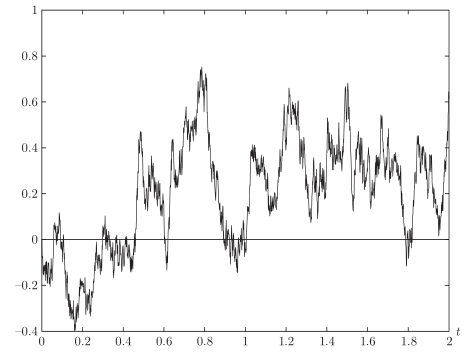
\includegraphics[scale=.45]{./graphics/wiener-trajectory.png}
      \caption{Wiener trajectory}
    \end{figure}

  }
\end{frame}

\begin{frame}
  \frametitle{Quadratic Variation}
  \begin{block}{Motivation}
    A stochastic process does not have the normal notion of variance.
  \end{block}
  \begin{definition}
    Suppose $P$ is a partition of $[0,t]$ denoted $t_k$ and let $\lVert P \rVert$ be the mesh of the partition then
        \begin{align*}
          [X]_t = \lim\limits_{\lVert P \rVert \to 0} \displaystyle\sum_{k = 1}^{n}(X_{t_k} - X_{t_{k-1}})^2
        \end{align*}
  \end{definition}
  \begin{block}{Comments}
    Note that Quadratic Variation itself is a stochastic process. An intuitive way to think about quadratic variation is the internal clock of a process, describing how randomness accumulates over time.
  \end{block}
\end{frame}

\begin{frame}
  \frametitle{Quadratic Variation of Wiener Process}
    \begin{theorem}
      Quadratic variation of a Wiener Process is $t$
    \end{theorem}
    \only<1>{
      \begin{block}{Proof}
        Let $P = \{0 = t_0 \leq t_1 \leq \dots \leq t_m = t\}$ be a partition of the interval $[0,t]$. Then the quadratic variation on $P$ is
      \begin{align*}
        [W]^{P} &= \displaystyle\sum_{k = 1}^{m}(W_{t_k} - W_{t_{k-1}})^2 
      \end{align*}
      Therefore,
      \begin{align*}
        E\left[[W]^{P}\right] &= \displaystyle\sum_{k = 1}^{m}E\left[(W_{t_k} - W_{t_{k-1}})^2\right]
      \end{align*}
      \end{block}
    }
    \only<2>{
      \begin{block}{Proof cont.}
      Note that $E[(W_{t_{i+1}} - W_{t_{i}})^2] = Var\left[W_{t_{i+1}} - W_{t_{i}}]$ such that
      \begin{align*}
        E\left[[W]^{P}\right] &= \displaystyle\sum_{k = 1}^{m}Var\left[W_{t_k} - W_{t_{k-1}}\right]
      \end{align*}
      It follows from the definition of the Wiener process that
      \begin{align*}
        E\left[[W]^{P}\right] &= \displaystyle\sum_{k = 1}^{m}(t_{k} - t_{k-1}) \\
        &= t
      \end{align*}
      \end{block}
    }
    \only<3>{
      \begin{proof}[Proof end]
        Finally, from the definition of discrete expectation we have that $E[[W]^{P}] \coloneqq \lim\limits_{\lVert P \rVert \to 0} [W]^{P} \coloneqq t$
      \end{proof}
      \begin{block}{Implications}
        This motivates us to write 
        \begin{align*}
          \int\limits_{0}^{t}(dW_t)^2 = t
        \end{align*}
        Or equivalently,
        \begin{align*}
          (dW_t)^2 = dt
        \end{align*}
      \end{block}

    }
\end{frame}

\begin{frame}
  \frametitle{Everything It$\hat{o}$}
\end{frame}

\begin{frame}
  \frametitle{The Stochastic Integral}
  \begin{block}{The Problem}
    Integrals of the form $\displaystyle\int_{0}^{t}g_s dW_s$.
  \end{block}
  \pause
  \only<2>{
    \begin{block}{Solution 1}
      Riemman Integral
      \begin{enumerate}
        \item $\displaystyle\sum_{k = 1}^{n}g_s(t_k)(W_{k+1} - W_{k})$
        \item Not possible due to locally unbounded variation
      \end{enumerate}
    \end{block}
  }
\end{frame}

\begin{frame}
  \frametitle{Geometric Brownian Motion Model}
  \only<1>{
  \begin{definition}
    \textbf{Geometric Brownian Motion} is a stochastic process whose dynamics follow the stochastic differential equation 
    \begin{align*}
      dX_t = \alpha X_t dt + \sigma X_t dW_t
    \end{align*}
    We can write the equation as 
    \begin{align*}
      X_t = (\alpha + \sigma W_t)X_t
    \end{align*}
    Where $W$ is the time derivative of the Wiener process.
  \end{definition}
  }
  \only<2>{
  \begin{block}{Derivation}
    Assume $S_t$ follows a Geometric Brownian Motion. Using Ito's lemma,
    \begin{align*}
      d\log(S_t) = \frac{1}{S_t}dS_t - \frac{1}{2S_t^2}(dSt)^2
    \end{align*}
    From the definition,
    \begin{align*}
      d\log(S_t) = \frac{1}{S_t}(\mu S_t dt + \sigma S_t dW_t) - \frac{1}{2S_t^2}(\mu S_t dt + \sigma S_t dW_t)^2 
    \end{align*}
    Note that
    \begin{align*}
      (\mu S_t dt + \sigma S_t dW_t)^2 &= S_t^2(\mu^2dt^2 + \sigma^2dW_t^2 + 2\mu \sigma dtdW_t)
    \end{align*}
    From Ito's multiplication table, $dt^2 = 0 = dtdW_t$ and $dW_t^2 = dt$ such that
    \begin{align*}
      (\mu S_t dt + \sigma S_t dW_t)^2 &= S_t^2 \sigma^2 dt
    \end{align*}
  \end{block}
  }
  \only<3>{
    \begin{block}{Derivation cont.}
      Substituting back,
      \begin{align*}
        dlog(S_t) &= (\mu dt + \sigma dW_t) - \frac{1}{2S_t^2}(S_t^2 \sigma^2 dt) \\
        &= (\mu - \frac{\sigma^2}{2})dt + \sigma dW_t
      \end{align*}
    \end{block}
  }
\end{frame}

\end{document}
